\documentclass{book}
\usepackage[a4paper,top=2.5cm,bottom=2.5cm,left=2.5cm,right=2.5cm]{geometry}
\usepackage{makeidx}
\usepackage{natbib}
\usepackage{graphicx}
\usepackage{multicol}
\usepackage{float}
\usepackage{listings}
\usepackage{color}
\usepackage{ifthen}
\usepackage[table]{xcolor}
\usepackage{textcomp}
\usepackage{alltt}
\usepackage{ifpdf}
\ifpdf
\usepackage[pdftex,
            pagebackref=true,
            colorlinks=true,
            linkcolor=blue,
            unicode
           ]{hyperref}
\else
\usepackage[ps2pdf,
            pagebackref=true,
            colorlinks=true,
            linkcolor=blue,
            unicode
           ]{hyperref}
\usepackage{pspicture}
\fi
\usepackage[utf8]{inputenc}
\usepackage{mathptmx}
\usepackage[scaled=.90]{helvet}
\usepackage{courier}
\usepackage{sectsty}
\usepackage{amssymb}
\usepackage[titles]{tocloft}
\usepackage{doxygen}
\lstset{language=C++,inputencoding=utf8,basicstyle=\footnotesize,breaklines=true,breakatwhitespace=true,tabsize=8,numbers=left }
\makeindex
\setcounter{tocdepth}{3}
\renewcommand{\footrulewidth}{0.4pt}
\renewcommand{\familydefault}{\sfdefault}
\hfuzz=15pt
\setlength{\emergencystretch}{15pt}
\hbadness=750
\tolerance=750
\begin{document}
\hypersetup{pageanchor=false,citecolor=blue}
\begin{titlepage}
\vspace*{7cm}
\begin{center}
{\Large libspire\-\_\-serial \\[1ex]\large 0.\-0.\-1 }\\
\vspace*{1cm}
{\large Generated by Doxygen 1.8.1.2}\\
\vspace*{0.5cm}
{\small Mon Jul 7 2014 18:54:10}\\
\end{center}
\end{titlepage}
\clearemptydoublepage
\pagenumbering{roman}
\tableofcontents
\clearemptydoublepage
\pagenumbering{arabic}
\hypersetup{pageanchor=true,citecolor=blue}
\chapter{libspire\-\_\-serial}
\label{md_README}
\hypertarget{md_README}{}
Library for communication with serial ports written in Vala (Windows -\/ Linux) 
\chapter{Namespace Index}
\section{Packages}
Here are the packages with brief descriptions (if available)\-:\begin{DoxyCompactList}
\item\contentsline{section}{\hyperlink{namespaceedwinspire}{edwinspire} }{\pageref{namespaceedwinspire}}{}
\item\contentsline{section}{\hyperlink{namespaceedwinspire_1_1_ports}{edwinspire\-::\-Ports} }{\pageref{namespaceedwinspire_1_1_ports}}{}
\end{DoxyCompactList}

\chapter{Class Index}
\section{Class Hierarchy}
This inheritance list is sorted roughly, but not completely, alphabetically\-:\begin{DoxyCompactList}
\item \contentsline{section}{edwinspire\-:\-:Ports\-:\-:Configure}{\pageref{classedwinspire_1_1_ports_1_1_configure}}{}
\item \contentsline{section}{edwinspire\-:\-:Ports\-:\-:Response}{\pageref{classedwinspire_1_1_ports_1_1_response}}{}
\item \contentsline{section}{Serial\-Port}{\pageref{class_serial_port}}{}
\begin{DoxyCompactList}
\item \contentsline{section}{edwinspire\-:\-:Ports\-:\-:Modem}{\pageref{classedwinspire_1_1_ports_1_1_modem}}{}
\end{DoxyCompactList}
\end{DoxyCompactList}

\chapter{Class Index}
\section{Class List}
Here are the classes, structs, unions and interfaces with brief descriptions\-:\begin{DoxyCompactList}
\item\contentsline{section}{\hyperlink{classedwinspire_1_1_ports_1_1_configure}{edwinspire\-::\-Ports\-::\-Configure} }{\pageref{classedwinspire_1_1_ports_1_1_configure}}{}
\item\contentsline{section}{\hyperlink{classedwinspire_1_1_ports_1_1_modem}{edwinspire\-::\-Ports\-::\-Modem} }{\pageref{classedwinspire_1_1_ports_1_1_modem}}{}
\item\contentsline{section}{\hyperlink{classedwinspire_1_1_ports_1_1_response}{edwinspire\-::\-Ports\-::\-Response} \\*Dummy class used for illustration purposes. Doing something with it }{\pageref{classedwinspire_1_1_ports_1_1_response}}{}
\item\contentsline{section}{\hyperlink{class_serial_port}{Serial\-Port} }{\pageref{class_serial_port}}{}
\end{DoxyCompactList}

\chapter{Namespace Documentation}
\hypertarget{namespaceedwinspire}{\section{edwinspire Namespace Reference}
\label{namespaceedwinspire}\index{edwinspire@{edwinspire}}
}
\subsection*{Packages}
\begin{DoxyCompactItemize}
\item 
namespace \hyperlink{namespaceedwinspire_1_1_ports}{Ports}
\end{DoxyCompactItemize}


\subsection{Detailed Description}
Namespace edwinspire covers the entire software developed by Edwin De La Cruz

\begin{DoxyAuthor}{Author}
Edwin De La Cruz 
\end{DoxyAuthor}

\hypertarget{namespaceedwinspire_1_1_ports}{\section{edwinspire\-:\-:Ports Namespace Reference}
\label{namespaceedwinspire_1_1_ports}\index{edwinspire\-::\-Ports@{edwinspire\-::\-Ports}}
}
\subsection*{Classes}
\begin{DoxyCompactItemize}
\item 
class \hyperlink{classedwinspire_1_1_ports_1_1_response}{Response}
\begin{DoxyCompactList}\small\item\em Dummy class used for illustration purposes. Doing something with it. \end{DoxyCompactList}\item 
class \hyperlink{classedwinspire_1_1_ports_1_1_modem}{Modem}
\item 
class \hyperlink{classedwinspire_1_1_ports_1_1_configure}{Configure}
\end{DoxyCompactItemize}
\subsection*{Enumerations}
\begin{DoxyCompactItemize}
\item 
enum \hyperlink{namespaceedwinspire_1_1_ports_ab404a94ffd8da908dfa277d25f4e5012}{Parity} \{ \\*
\hyperlink{namespaceedwinspire_1_1_ports_afd526aa1ebf856f40b0dfdbef71f7077a84b2ed1a0b5fa1c47adc8f831ab31905}{N\-O\-N\-E}, 
\hyperlink{namespaceedwinspire_1_1_ports_ab404a94ffd8da908dfa277d25f4e5012ac23034d2e91faad9fdd2622dc18ea68a}{O\-D\-D}, 
\hyperlink{namespaceedwinspire_1_1_ports_ab404a94ffd8da908dfa277d25f4e5012a92d49491abed377cf965b3f92fc1db93}{E\-V\-E\-N}, 
\hyperlink{namespaceedwinspire_1_1_ports_ab404a94ffd8da908dfa277d25f4e5012a718d74fa16efccda38efe9777f85182c}{M\-A\-R\-K}, 
\\*
\hyperlink{namespaceedwinspire_1_1_ports_ab404a94ffd8da908dfa277d25f4e5012ab48f2b83ab49826899006555f7b42f10}{S\-P\-A\-C\-E}
 \}
\item 
enum \hyperlink{namespaceedwinspire_1_1_ports_afd526aa1ebf856f40b0dfdbef71f7077}{Hand\-Shaking} \{ \hyperlink{namespaceedwinspire_1_1_ports_afd526aa1ebf856f40b0dfdbef71f7077a84b2ed1a0b5fa1c47adc8f831ab31905}{N\-O\-N\-E}, 
\hyperlink{namespaceedwinspire_1_1_ports_afd526aa1ebf856f40b0dfdbef71f7077a46872380b7a1a604c61aa0476c13cc17}{R\-T\-S\-\_\-\-C\-T\-S}, 
\hyperlink{namespaceedwinspire_1_1_ports_afd526aa1ebf856f40b0dfdbef71f7077a138f62dafca279af31d78f4874622b8c}{X\-On\-X\-Off}, 
\hyperlink{namespaceedwinspire_1_1_ports_afd526aa1ebf856f40b0dfdbef71f7077ac6ecd9358e9373acb9718d6853d78e4b}{D\-T\-R\-\_\-\-D\-S\-R}
 \}
\item 
enum \hyperlink{namespaceedwinspire_1_1_ports_a8f46ab15ec2741c3e028c5c5ddff36d3}{Data\-Status} \{ \hyperlink{namespaceedwinspire_1_1_ports_a8f46ab15ec2741c3e028c5c5ddff36d3ab81c145f75c6ff159a38f7dc7fa76aed}{None}, 
{\bfseries Sending}, 
{\bfseries Receiving}
 \}
\item 
enum \hyperlink{namespaceedwinspire_1_1_ports_ac176c111882ba8478fef22b8f15a22b5}{Response\-Code} \{ \\*
\hyperlink{namespaceedwinspire_1_1_ports_ac176c111882ba8478fef22b8f15a22b5a1645bd09cf62925e0927475c8000e53c}{O\-K} =  0, 
\hyperlink{namespaceedwinspire_1_1_ports_ac176c111882ba8478fef22b8f15a22b5adfbca35fcb8c3f5ed08552ae8e880a41}{C\-O\-N\-N\-E\-C\-T} =  1, 
\hyperlink{namespaceedwinspire_1_1_ports_ac176c111882ba8478fef22b8f15a22b5ad2e40384ffb938077ec7e364d6fa8095}{R\-I\-N\-G} =  2, 
\hyperlink{namespaceedwinspire_1_1_ports_ac176c111882ba8478fef22b8f15a22b5acde6524b1a18be2842ea9d46e42a6073}{N\-O\-C\-A\-R\-R\-I\-E\-R} =  3, 
\\*
\hyperlink{namespaceedwinspire_1_1_ports_ac176c111882ba8478fef22b8f15a22b5a9ff899bf11a96eb22b333dd7a2961a72}{E\-R\-R\-O\-R} =  4, 
\hyperlink{namespaceedwinspire_1_1_ports_ac176c111882ba8478fef22b8f15a22b5a9b5fdc8d8b446c33e1cb4ae879a806df}{N\-O\-D\-I\-A\-L\-T\-O\-N\-E} =  5, 
\hyperlink{namespaceedwinspire_1_1_ports_ac176c111882ba8478fef22b8f15a22b5aba8beeb5bf4bbac05da73e134afc505e}{B\-U\-S\-Y} =  6, 
\hyperlink{namespaceedwinspire_1_1_ports_ac176c111882ba8478fef22b8f15a22b5aaf85258a688895edef1ff43971b72552}{N\-O\-A\-N\-S\-W\-E\-R} =  7, 
\\*
\hyperlink{namespaceedwinspire_1_1_ports_ac176c111882ba8478fef22b8f15a22b5a54f22d2adb23016fb70d1e06dcea5cb2}{E\-R\-R\-O\-R\-\_\-\-C\-M\-S} =  98, 
\hyperlink{namespaceedwinspire_1_1_ports_ac176c111882ba8478fef22b8f15a22b5a328ffb4f9de9644b4932a4a43b50b954}{E\-R\-R\-O\-R\-\_\-\-C\-M\-E} =  99, 
{\bfseries U\-N\-K\-N\-O\-W} =  100
 \}
\end{DoxyCompactItemize}
\subsection*{Functions}
\begin{DoxyCompactItemize}
\item 
public enum \\*
\hyperlink{namespaceedwinspire_1_1_ports_ab404a94ffd8da908dfa277d25f4e5012}{edwinspire\-::\-Ports\-::\-Parity} \hyperlink{namespaceedwinspire_1_1_ports_a3b5ab9c73da132e47d164f322cf54904}{Description} (nick=\char`\"{}C\-M\-S\char`\"{}, blurb=\char`\"{}These are the error codes for +C\-M\-S \hyperlink{namespaceedwinspire_1_1_ports_ac176c111882ba8478fef22b8f15a22b5a9ff899bf11a96eb22b333dd7a2961a72}{E\-R\-R\-O\-R}\char`\"{})\mbox{]} public enum C\-M\-S
\item 
\hypertarget{namespaceedwinspire_1_1_ports_a1cb04d0401c5f2277711b286f3199061}{public {\bfseries Last\-Call\-Received} ()}\label{namespaceedwinspire_1_1_ports_a1cb04d0401c5f2277711b286f3199061}

\item 
\hypertarget{namespaceedwinspire_1_1_ports_a10704194579fb04d8727a79a98d53f3f}{{\bfseries Status} (\hyperlink{namespaceedwinspire_1_1_ports_a8f46ab15ec2741c3e028c5c5ddff36d3}{Data\-Status} Status)}\label{namespaceedwinspire_1_1_ports_a10704194579fb04d8727a79a98d53f3f}

\item 
\hypertarget{namespaceedwinspire_1_1_ports_a9de2452f18841a5338e2c45fbc8cca2d}{public \hyperlink{class_serial_port}{Serial\-Port} {\bfseries with\-\_\-args} (string Port\-\_\-=\char`\"{}/dev/tty\-S0\char`\"{}, uint Baudrate=2400, uint Data\-Bits=8, \hyperlink{namespaceedwinspire_1_1_ports_ab404a94ffd8da908dfa277d25f4e5012}{Parity} Parity\-\_\-=Parity.\-N\-O\-N\-E, Stop\-Bits Stop\-Bits\-\_\-=Stop\-Bits.\-O\-N\-E, \hyperlink{namespaceedwinspire_1_1_ports_afd526aa1ebf856f40b0dfdbef71f7077}{Hand\-Shaking} H\-S\-\_\-=Hand\-Shaking.\-N\-O\-N\-E)}\label{namespaceedwinspire_1_1_ports_a9de2452f18841a5338e2c45fbc8cca2d}

\item 
\hypertarget{namespaceedwinspire_1_1_ports_af8d9afe49636a2f0ba22f1f17bbaba17}{private void {\bfseries connect\-Signals} ()}\label{namespaceedwinspire_1_1_ports_af8d9afe49636a2f0ba22f1f17bbaba17}

\item 
\hypertarget{namespaceedwinspire_1_1_ports_a293ef58b4105463e6bd4b2d5ad9b3144}{public {\bfseries Serial\-Port} ()}\label{namespaceedwinspire_1_1_ports_a293ef58b4105463e6bd4b2d5ad9b3144}

\item 
\hypertarget{namespaceedwinspire_1_1_ports_a17877b618445a0e65f46c94bc80bc821}{private bool {\bfseries Set\-\_\-\-Port} ()}\label{namespaceedwinspire_1_1_ports_a17877b618445a0e65f46c94bc80bc821}

\item 
\hypertarget{namespaceedwinspire_1_1_ports_ab4f5440159397421d6f1985dccda8aa7}{private bool {\bfseries Set} ()}\label{namespaceedwinspire_1_1_ports_ab4f5440159397421d6f1985dccda8aa7}

\item 
\hypertarget{namespaceedwinspire_1_1_ports_a7a08c939ddf6ae7e1426b3bd061c3f13}{private bool {\bfseries Setup\-\_\-\-Buffer\-\_\-} (ulong Buffer\-In, ulong Buffer\-Out)}\label{namespaceedwinspire_1_1_ports_a7a08c939ddf6ae7e1426b3bd061c3f13}

\item 
\hypertarget{namespaceedwinspire_1_1_ports_a16c386569d50ef1f47b43bce24c54cde}{private bool {\bfseries set\-\_\-handshaking} ()}\label{namespaceedwinspire_1_1_ports_a16c386569d50ef1f47b43bce24c54cde}

\item 
\hypertarget{namespaceedwinspire_1_1_ports_ae3a4888c33e46ef2cb9c21475b39747d}{public bool {\bfseries Discard\-Buffer} ()}\label{namespaceedwinspire_1_1_ports_ae3a4888c33e46ef2cb9c21475b39747d}

\item 
\hypertarget{namespaceedwinspire_1_1_ports_ab6cd9fa85820a8013aa6f47c89eb8102}{public string\mbox{[}$\,$\mbox{]} {\bfseries Get\-\_\-\-Port\-Name} ()}\label{namespaceedwinspire_1_1_ports_ab6cd9fa85820a8013aa6f47c89eb8102}

\end{DoxyCompactItemize}
\subsection*{Variables}
\begin{DoxyCompactItemize}
\item 
\hypertarget{namespaceedwinspire_1_1_ports_a809bb99c77e120d0d3e305149731746c}{\hyperlink{classedwinspire_1_1_ports_1_1_response}{edwinspire\-::\-Ports\-::\-Response} {\bfseries Number}}\label{namespaceedwinspire_1_1_ports_a809bb99c77e120d0d3e305149731746c}

\item 
\hypertarget{namespaceedwinspire_1_1_ports_a85143858f34117053e5460d22df04df8}{public Date\-Time {\bfseries Date}}\label{namespaceedwinspire_1_1_ports_a85143858f34117053e5460d22df04df8}

\item 
\hypertarget{namespaceedwinspire_1_1_ports_a5efed4bf03757ef2f2356e4d58bc0b25}{public bool {\bfseries Read}}\label{namespaceedwinspire_1_1_ports_a5efed4bf03757ef2f2356e4d58bc0b25}

\item 
\hypertarget{namespaceedwinspire_1_1_ports_a7f31b8084b1c093dde91fd7d442f0c33}{private int {\bfseries Gestor} = -\/1}\label{namespaceedwinspire_1_1_ports_a7f31b8084b1c093dde91fd7d442f0c33}

\item 
\hypertarget{namespaceedwinspire_1_1_ports_a2da87d6ac29df3f3ae83c405a4cfcd0f}{private bool {\bfseries Bloqueante} = false}\label{namespaceedwinspire_1_1_ports_a2da87d6ac29df3f3ae83c405a4cfcd0f}

\item 
\hypertarget{namespaceedwinspire_1_1_ports_a511c71a745dc25f1cec7d9b3977c1029}{private Timer {\bfseries Temporizador\-Interno\-Read\-Char} = new Timer()}\label{namespaceedwinspire_1_1_ports_a511c71a745dc25f1cec7d9b3977c1029}

\item 
\hypertarget{namespaceedwinspire_1_1_ports_a3fcb86d18a35e8e4926c82ffa679911a}{private Timer {\bfseries Temporizador\-Interno\-Read\-Line} = new Timer()}\label{namespaceedwinspire_1_1_ports_a3fcb86d18a35e8e4926c82ffa679911a}

\item 
\hypertarget{namespaceedwinspire_1_1_ports_a572884312471246cd0581385d6ce5abd}{private String\-Builder {\bfseries Linea\-Modem} = new String\-Builder()}\label{namespaceedwinspire_1_1_ports_a572884312471246cd0581385d6ce5abd}

\item 
\hypertarget{namespaceedwinspire_1_1_ports_a2d90f7f91e2a32b3ba4885640203178a}{public bool {\bfseries Log\-Modem} = false}\label{namespaceedwinspire_1_1_ports_a2d90f7f91e2a32b3ba4885640203178a}

\end{DoxyCompactItemize}


\subsection{Detailed Description}
Namespace \hyperlink{namespaceedwinspire_1_1_ports}{Ports} covers everything related to communications with serial ports 

\subsection{Enumeration Type Documentation}
\hypertarget{namespaceedwinspire_1_1_ports_a8f46ab15ec2741c3e028c5c5ddff36d3}{\index{edwinspire\-::\-Ports@{edwinspire\-::\-Ports}!Data\-Status@{Data\-Status}}
\index{Data\-Status@{Data\-Status}!edwinspire::Ports@{edwinspire\-::\-Ports}}
\subsubsection[{Data\-Status}]{\setlength{\rightskip}{0pt plus 5cm}enum {\bf edwinspire\-::\-Ports\-::\-Data\-Status}}}\label{namespaceedwinspire_1_1_ports_a8f46ab15ec2741c3e028c5c5ddff36d3}
\begin{Desc}
\item[Enumerator\-: ]\par
\begin{description}
\index{None@{None}!edwinspire\-::\-Ports@{edwinspire\-::\-Ports}}\index{edwinspire\-::\-Ports@{edwinspire\-::\-Ports}!None@{None}}\item[{\em 
\hypertarget{namespaceedwinspire_1_1_ports_a8f46ab15ec2741c3e028c5c5ddff36d3ab81c145f75c6ff159a38f7dc7fa76aed}{None}\label{namespaceedwinspire_1_1_ports_a8f46ab15ec2741c3e028c5c5ddff36d3ab81c145f75c6ff159a38f7dc7fa76aed}
}]None \end{description}
\end{Desc}



Definition at line 99 of file enum.\-vala.


\begin{DoxyCode}
                                       \{
                        [\hyperlink{namespaceedwinspire_1_1_ports_a3b5ab9c73da132e47d164f322cf54904}{Description}(nick = \textcolor{stringliteral}{"None"}, blurb = \textcolor{stringliteral}{"Modem
       no eta realizando ninguna accion"})]
                        None,  
                        [\hyperlink{namespaceedwinspire_1_1_ports_a3b5ab9c73da132e47d164f322cf54904}{Description}(nick = \textcolor{stringliteral}{"Sending"}, blurb = \textcolor{stringliteral}{"
      Enviando datos al modem"})]
                        Sending, 
                        [\hyperlink{namespaceedwinspire_1_1_ports_a3b5ab9c73da132e47d164f322cf54904}{Description}(nick = \textcolor{stringliteral}{"Receiving"}, blurb = \textcolor{stringliteral}{"
      Recibiendo datos del modem"})]
                        Receiving
                \}
\end{DoxyCode}
\hypertarget{namespaceedwinspire_1_1_ports_afd526aa1ebf856f40b0dfdbef71f7077}{\index{edwinspire\-::\-Ports@{edwinspire\-::\-Ports}!Hand\-Shaking@{Hand\-Shaking}}
\index{Hand\-Shaking@{Hand\-Shaking}!edwinspire::Ports@{edwinspire\-::\-Ports}}
\subsubsection[{Hand\-Shaking}]{\setlength{\rightskip}{0pt plus 5cm}enum {\bf edwinspire\-::\-Ports\-::\-Hand\-Shaking}}}\label{namespaceedwinspire_1_1_ports_afd526aa1ebf856f40b0dfdbef71f7077}
\begin{Desc}
\item[Enumerator\-: ]\par
\begin{description}
\index{N\-O\-N\-E@{N\-O\-N\-E}!edwinspire\-::\-Ports@{edwinspire\-::\-Ports}}\index{edwinspire\-::\-Ports@{edwinspire\-::\-Ports}!N\-O\-N\-E@{N\-O\-N\-E}}\item[{\em 
\hypertarget{namespaceedwinspire_1_1_ports_afd526aa1ebf856f40b0dfdbef71f7077a84b2ed1a0b5fa1c47adc8f831ab31905}{N\-O\-N\-E}\label{namespaceedwinspire_1_1_ports_afd526aa1ebf856f40b0dfdbef71f7077a84b2ed1a0b5fa1c47adc8f831ab31905}
}]None \index{R\-T\-S\-\_\-\-C\-T\-S@{R\-T\-S\-\_\-\-C\-T\-S}!edwinspire\-::\-Ports@{edwinspire\-::\-Ports}}\index{edwinspire\-::\-Ports@{edwinspire\-::\-Ports}!R\-T\-S\-\_\-\-C\-T\-S@{R\-T\-S\-\_\-\-C\-T\-S}}\item[{\em 
\hypertarget{namespaceedwinspire_1_1_ports_afd526aa1ebf856f40b0dfdbef71f7077a46872380b7a1a604c61aa0476c13cc17}{R\-T\-S\-\_\-\-C\-T\-S}\label{namespaceedwinspire_1_1_ports_afd526aa1ebf856f40b0dfdbef71f7077a46872380b7a1a604c61aa0476c13cc17}
}]R\-T\-S-\/\-C\-T\-S \index{X\-On\-X\-Off@{X\-On\-X\-Off}!edwinspire\-::\-Ports@{edwinspire\-::\-Ports}}\index{edwinspire\-::\-Ports@{edwinspire\-::\-Ports}!X\-On\-X\-Off@{X\-On\-X\-Off}}\item[{\em 
\hypertarget{namespaceedwinspire_1_1_ports_afd526aa1ebf856f40b0dfdbef71f7077a138f62dafca279af31d78f4874622b8c}{X\-On\-X\-Off}\label{namespaceedwinspire_1_1_ports_afd526aa1ebf856f40b0dfdbef71f7077a138f62dafca279af31d78f4874622b8c}
}]X\-On\-X\-Off \index{D\-T\-R\-\_\-\-D\-S\-R@{D\-T\-R\-\_\-\-D\-S\-R}!edwinspire\-::\-Ports@{edwinspire\-::\-Ports}}\index{edwinspire\-::\-Ports@{edwinspire\-::\-Ports}!D\-T\-R\-\_\-\-D\-S\-R@{D\-T\-R\-\_\-\-D\-S\-R}}\item[{\em 
\hypertarget{namespaceedwinspire_1_1_ports_afd526aa1ebf856f40b0dfdbef71f7077ac6ecd9358e9373acb9718d6853d78e4b}{D\-T\-R\-\_\-\-D\-S\-R}\label{namespaceedwinspire_1_1_ports_afd526aa1ebf856f40b0dfdbef71f7077ac6ecd9358e9373acb9718d6853d78e4b}
}]D\-T\-R-\/\-D\-S\-R \end{description}
\end{Desc}



Definition at line 74 of file enum.\-vala.


\begin{DoxyCode}
                                       \{
                        [\hyperlink{namespaceedwinspire_1_1_ports_a3b5ab9c73da132e47d164f322cf54904}{Description}(nick = \textcolor{stringliteral}{"NONE"}, blurb = \textcolor{stringliteral}{"No se
       utiliza ningun control para el protocol de enlace"})]
                        NONE, 
                        [\hyperlink{namespaceedwinspire_1_1_ports_a3b5ab9c73da132e47d164f322cf54904}{Description}(nick = \textcolor{stringliteral}{"RTS-CTS"}, blurb = \textcolor{stringliteral}{"
      Controles por hardware, Solicitud de encio (RTS) y Listo para enviar (CTS)"})]
                        RTS\_CTS, 
                        [\hyperlink{namespaceedwinspire_1_1_ports_a3b5ab9c73da132e47d164f322cf54904}{Description}(nick = \textcolor{stringliteral}{"XOnXOff"}, blurb = \textcolor{stringliteral}{"
      Protocolo de control de software XON/XOFF"})]
                        XOnXOff, 
                        [\hyperlink{namespaceedwinspire_1_1_ports_a3b5ab9c73da132e47d164f322cf54904}{Description}(nick = \textcolor{stringliteral}{"DTR-DSR"}, blurb = \textcolor{stringliteral}{"
      Utiliza tanto RTS CTS como XON/XOFF"})]
                        DTR\_DSR  
                \}
\end{DoxyCode}
\hypertarget{namespaceedwinspire_1_1_ports_ab404a94ffd8da908dfa277d25f4e5012}{\index{edwinspire\-::\-Ports@{edwinspire\-::\-Ports}!Parity@{Parity}}
\index{Parity@{Parity}!edwinspire::Ports@{edwinspire\-::\-Ports}}
\subsubsection[{Parity}]{\setlength{\rightskip}{0pt plus 5cm}enum {\bf edwinspire\-::\-Ports\-::\-Parity}}}\label{namespaceedwinspire_1_1_ports_ab404a94ffd8da908dfa277d25f4e5012}
\begin{Desc}
\item[Enumerator\-: ]\par
\begin{description}
\index{N\-O\-N\-E@{N\-O\-N\-E}!edwinspire\-::\-Ports@{edwinspire\-::\-Ports}}\index{edwinspire\-::\-Ports@{edwinspire\-::\-Ports}!N\-O\-N\-E@{N\-O\-N\-E}}\item[{\em 
\hypertarget{namespaceedwinspire_1_1_ports_afd526aa1ebf856f40b0dfdbef71f7077a84b2ed1a0b5fa1c47adc8f831ab31905}{N\-O\-N\-E}\label{namespaceedwinspire_1_1_ports_afd526aa1ebf856f40b0dfdbef71f7077a84b2ed1a0b5fa1c47adc8f831ab31905}
}]None \index{O\-D\-D@{O\-D\-D}!edwinspire\-::\-Ports@{edwinspire\-::\-Ports}}\index{edwinspire\-::\-Ports@{edwinspire\-::\-Ports}!O\-D\-D@{O\-D\-D}}\item[{\em 
\hypertarget{namespaceedwinspire_1_1_ports_ab404a94ffd8da908dfa277d25f4e5012ac23034d2e91faad9fdd2622dc18ea68a}{O\-D\-D}\label{namespaceedwinspire_1_1_ports_ab404a94ffd8da908dfa277d25f4e5012ac23034d2e91faad9fdd2622dc18ea68a}
}]Odd \index{E\-V\-E\-N@{E\-V\-E\-N}!edwinspire\-::\-Ports@{edwinspire\-::\-Ports}}\index{edwinspire\-::\-Ports@{edwinspire\-::\-Ports}!E\-V\-E\-N@{E\-V\-E\-N}}\item[{\em 
\hypertarget{namespaceedwinspire_1_1_ports_ab404a94ffd8da908dfa277d25f4e5012a92d49491abed377cf965b3f92fc1db93}{E\-V\-E\-N}\label{namespaceedwinspire_1_1_ports_ab404a94ffd8da908dfa277d25f4e5012a92d49491abed377cf965b3f92fc1db93}
}]Even \index{M\-A\-R\-K@{M\-A\-R\-K}!edwinspire\-::\-Ports@{edwinspire\-::\-Ports}}\index{edwinspire\-::\-Ports@{edwinspire\-::\-Ports}!M\-A\-R\-K@{M\-A\-R\-K}}\item[{\em 
\hypertarget{namespaceedwinspire_1_1_ports_ab404a94ffd8da908dfa277d25f4e5012a718d74fa16efccda38efe9777f85182c}{M\-A\-R\-K}\label{namespaceedwinspire_1_1_ports_ab404a94ffd8da908dfa277d25f4e5012a718d74fa16efccda38efe9777f85182c}
}]Mark \index{S\-P\-A\-C\-E@{S\-P\-A\-C\-E}!edwinspire\-::\-Ports@{edwinspire\-::\-Ports}}\index{edwinspire\-::\-Ports@{edwinspire\-::\-Ports}!S\-P\-A\-C\-E@{S\-P\-A\-C\-E}}\item[{\em 
\hypertarget{namespaceedwinspire_1_1_ports_ab404a94ffd8da908dfa277d25f4e5012ab48f2b83ab49826899006555f7b42f10}{S\-P\-A\-C\-E}\label{namespaceedwinspire_1_1_ports_ab404a94ffd8da908dfa277d25f4e5012ab48f2b83ab49826899006555f7b42f10}
}]Space \end{description}
\end{Desc}



Definition at line 31 of file enum.\-vala.


\begin{DoxyCode}
                           \{
                        [\hyperlink{namespaceedwinspire_1_1_ports_a3b5ab9c73da132e47d164f322cf54904}{Description}(nick = \textcolor{stringliteral}{"NONE"}, blurb = \textcolor{stringliteral}{"No se
       produce una comprobación de paridad"})]
                        NONE,  
                        [\hyperlink{namespaceedwinspire_1_1_ports_a3b5ab9c73da132e47d164f322cf54904}{Description}(nick = \textcolor{stringliteral}{"ODD"}, blurb = \textcolor{stringliteral}{"
      Establece el bit de paridad de forma que el recuento de bits establecidos sea un número
       impar"})]
                        ODD,  
                        [\hyperlink{namespaceedwinspire_1_1_ports_a3b5ab9c73da132e47d164f322cf54904}{Description}(nick = \textcolor{stringliteral}{"EVEN"}, blurb = \textcolor{stringliteral}{"
      Establece el bit de paridad de forma que el recuento de bits establecidos sea un número
       par"})]
                        EVEN,  
                        [\hyperlink{namespaceedwinspire_1_1_ports_a3b5ab9c73da132e47d164f322cf54904}{Description}(nick = \textcolor{stringliteral}{"MARK"}, blurb = \textcolor{stringliteral}{"
      Establece el conjunto de bits de paridad en 1"})]
                        MARK,  
                        [\hyperlink{namespaceedwinspire_1_1_ports_a3b5ab9c73da132e47d164f322cf54904}{Description}(nick = \textcolor{stringliteral}{"SPACE"}, blurb = \textcolor{stringliteral}{"
      Establece el conjunto de bits de paridad en 0"})]
                        SPACE  
                \}               
\end{DoxyCode}
\hypertarget{namespaceedwinspire_1_1_ports_ac176c111882ba8478fef22b8f15a22b5}{\index{edwinspire\-::\-Ports@{edwinspire\-::\-Ports}!Response\-Code@{Response\-Code}}
\index{Response\-Code@{Response\-Code}!edwinspire::Ports@{edwinspire\-::\-Ports}}
\subsubsection[{Response\-Code}]{\setlength{\rightskip}{0pt plus 5cm}enum {\bf edwinspire\-::\-Ports\-::\-Response\-Code}}}\label{namespaceedwinspire_1_1_ports_ac176c111882ba8478fef22b8f15a22b5}
\begin{Desc}
\item[Enumerator\-: ]\par
\begin{description}
\index{O\-K@{O\-K}!edwinspire\-::\-Ports@{edwinspire\-::\-Ports}}\index{edwinspire\-::\-Ports@{edwinspire\-::\-Ports}!O\-K@{O\-K}}\item[{\em 
\hypertarget{namespaceedwinspire_1_1_ports_ac176c111882ba8478fef22b8f15a22b5a1645bd09cf62925e0927475c8000e53c}{O\-K}\label{namespaceedwinspire_1_1_ports_ac176c111882ba8478fef22b8f15a22b5a1645bd09cf62925e0927475c8000e53c}
}]\hyperlink{classedwinspire_1_1_ports_1_1_modem}{Modem} response O\-K \index{C\-O\-N\-N\-E\-C\-T@{C\-O\-N\-N\-E\-C\-T}!edwinspire\-::\-Ports@{edwinspire\-::\-Ports}}\index{edwinspire\-::\-Ports@{edwinspire\-::\-Ports}!C\-O\-N\-N\-E\-C\-T@{C\-O\-N\-N\-E\-C\-T}}\item[{\em 
\hypertarget{namespaceedwinspire_1_1_ports_ac176c111882ba8478fef22b8f15a22b5adfbca35fcb8c3f5ed08552ae8e880a41}{C\-O\-N\-N\-E\-C\-T}\label{namespaceedwinspire_1_1_ports_ac176c111882ba8478fef22b8f15a22b5adfbca35fcb8c3f5ed08552ae8e880a41}
}]Connect \index{R\-I\-N\-G@{R\-I\-N\-G}!edwinspire\-::\-Ports@{edwinspire\-::\-Ports}}\index{edwinspire\-::\-Ports@{edwinspire\-::\-Ports}!R\-I\-N\-G@{R\-I\-N\-G}}\item[{\em 
\hypertarget{namespaceedwinspire_1_1_ports_ac176c111882ba8478fef22b8f15a22b5ad2e40384ffb938077ec7e364d6fa8095}{R\-I\-N\-G}\label{namespaceedwinspire_1_1_ports_ac176c111882ba8478fef22b8f15a22b5ad2e40384ffb938077ec7e364d6fa8095}
}]Ring \index{N\-O\-C\-A\-R\-R\-I\-E\-R@{N\-O\-C\-A\-R\-R\-I\-E\-R}!edwinspire\-::\-Ports@{edwinspire\-::\-Ports}}\index{edwinspire\-::\-Ports@{edwinspire\-::\-Ports}!N\-O\-C\-A\-R\-R\-I\-E\-R@{N\-O\-C\-A\-R\-R\-I\-E\-R}}\item[{\em 
\hypertarget{namespaceedwinspire_1_1_ports_ac176c111882ba8478fef22b8f15a22b5acde6524b1a18be2842ea9d46e42a6073}{N\-O\-C\-A\-R\-R\-I\-E\-R}\label{namespaceedwinspire_1_1_ports_ac176c111882ba8478fef22b8f15a22b5acde6524b1a18be2842ea9d46e42a6073}
}]No carrier \index{E\-R\-R\-O\-R@{E\-R\-R\-O\-R}!edwinspire\-::\-Ports@{edwinspire\-::\-Ports}}\index{edwinspire\-::\-Ports@{edwinspire\-::\-Ports}!E\-R\-R\-O\-R@{E\-R\-R\-O\-R}}\item[{\em 
\hypertarget{namespaceedwinspire_1_1_ports_ac176c111882ba8478fef22b8f15a22b5a9ff899bf11a96eb22b333dd7a2961a72}{E\-R\-R\-O\-R}\label{namespaceedwinspire_1_1_ports_ac176c111882ba8478fef22b8f15a22b5a9ff899bf11a96eb22b333dd7a2961a72}
}]Error \index{N\-O\-D\-I\-A\-L\-T\-O\-N\-E@{N\-O\-D\-I\-A\-L\-T\-O\-N\-E}!edwinspire\-::\-Ports@{edwinspire\-::\-Ports}}\index{edwinspire\-::\-Ports@{edwinspire\-::\-Ports}!N\-O\-D\-I\-A\-L\-T\-O\-N\-E@{N\-O\-D\-I\-A\-L\-T\-O\-N\-E}}\item[{\em 
\hypertarget{namespaceedwinspire_1_1_ports_ac176c111882ba8478fef22b8f15a22b5a9b5fdc8d8b446c33e1cb4ae879a806df}{N\-O\-D\-I\-A\-L\-T\-O\-N\-E}\label{namespaceedwinspire_1_1_ports_ac176c111882ba8478fef22b8f15a22b5a9b5fdc8d8b446c33e1cb4ae879a806df}
}]No dial tone \index{B\-U\-S\-Y@{B\-U\-S\-Y}!edwinspire\-::\-Ports@{edwinspire\-::\-Ports}}\index{edwinspire\-::\-Ports@{edwinspire\-::\-Ports}!B\-U\-S\-Y@{B\-U\-S\-Y}}\item[{\em 
\hypertarget{namespaceedwinspire_1_1_ports_ac176c111882ba8478fef22b8f15a22b5aba8beeb5bf4bbac05da73e134afc505e}{B\-U\-S\-Y}\label{namespaceedwinspire_1_1_ports_ac176c111882ba8478fef22b8f15a22b5aba8beeb5bf4bbac05da73e134afc505e}
}]Busy \index{N\-O\-A\-N\-S\-W\-E\-R@{N\-O\-A\-N\-S\-W\-E\-R}!edwinspire\-::\-Ports@{edwinspire\-::\-Ports}}\index{edwinspire\-::\-Ports@{edwinspire\-::\-Ports}!N\-O\-A\-N\-S\-W\-E\-R@{N\-O\-A\-N\-S\-W\-E\-R}}\item[{\em 
\hypertarget{namespaceedwinspire_1_1_ports_ac176c111882ba8478fef22b8f15a22b5aaf85258a688895edef1ff43971b72552}{N\-O\-A\-N\-S\-W\-E\-R}\label{namespaceedwinspire_1_1_ports_ac176c111882ba8478fef22b8f15a22b5aaf85258a688895edef1ff43971b72552}
}]No answer \index{E\-R\-R\-O\-R\-\_\-\-C\-M\-S@{E\-R\-R\-O\-R\-\_\-\-C\-M\-S}!edwinspire\-::\-Ports@{edwinspire\-::\-Ports}}\index{edwinspire\-::\-Ports@{edwinspire\-::\-Ports}!E\-R\-R\-O\-R\-\_\-\-C\-M\-S@{E\-R\-R\-O\-R\-\_\-\-C\-M\-S}}\item[{\em 
\hypertarget{namespaceedwinspire_1_1_ports_ac176c111882ba8478fef22b8f15a22b5a54f22d2adb23016fb70d1e06dcea5cb2}{E\-R\-R\-O\-R\-\_\-\-C\-M\-S}\label{namespaceedwinspire_1_1_ports_ac176c111882ba8478fef22b8f15a22b5a54f22d2adb23016fb70d1e06dcea5cb2}
}]Modems G\-S\-M response with Error \index{E\-R\-R\-O\-R\-\_\-\-C\-M\-E@{E\-R\-R\-O\-R\-\_\-\-C\-M\-E}!edwinspire\-::\-Ports@{edwinspire\-::\-Ports}}\index{edwinspire\-::\-Ports@{edwinspire\-::\-Ports}!E\-R\-R\-O\-R\-\_\-\-C\-M\-E@{E\-R\-R\-O\-R\-\_\-\-C\-M\-E}}\item[{\em 
\hypertarget{namespaceedwinspire_1_1_ports_ac176c111882ba8478fef22b8f15a22b5a328ffb4f9de9644b4932a4a43b50b954}{E\-R\-R\-O\-R\-\_\-\-C\-M\-E}\label{namespaceedwinspire_1_1_ports_ac176c111882ba8478fef22b8f15a22b5a328ffb4f9de9644b4932a4a43b50b954}
}]C\-M\-E response with error \end{description}
\end{Desc}



Definition at line 148 of file enum.\-vala.


\begin{DoxyCode}
                                         \{
                        OK = 0, 
                        CONNECT = 1, 
                        RING = 2, 
                        NOCARRIER = 3, 
                        ERROR = 4, 
                        NODIALTONE = 5, 
                        BUSY = 6, 
                        NOANSWER = 7, 
                        [\hyperlink{namespaceedwinspire_1_1_ports_a3b5ab9c73da132e47d164f322cf54904}{Description}(nick = \textcolor{stringliteral}{"ERROR CMS"}, blurb = \textcolor{stringliteral}{"
      Responde con ERROR modem GSM"})]
                        ERROR\_CMS = 98, 
                        [\hyperlink{namespaceedwinspire_1_1_ports_a3b5ab9c73da132e47d164f322cf54904}{Description}(nick = \textcolor{stringliteral}{"ERROR CME"}, blurb = \textcolor{stringliteral}{"
      Responde con ERROR CME"})]
                        ERROR\_CME = 99, 
                        UNKNOW = 100
                \}
\end{DoxyCode}


\subsection{Function Documentation}
\hypertarget{namespaceedwinspire_1_1_ports_a3b5ab9c73da132e47d164f322cf54904}{\index{edwinspire\-::\-Ports@{edwinspire\-::\-Ports}!Description@{Description}}
\index{Description@{Description}!edwinspire::Ports@{edwinspire\-::\-Ports}}
\subsubsection[{Description}]{\setlength{\rightskip}{0pt plus 5cm}public enum {\bf edwinspire\-::\-Ports\-::\-Response\-Code} edwinspire\-::\-Ports\-::\-Description (
\begin{DoxyParamCaption}
\item[{nick}]{ = {\ttfamily \char`\"{}CMS\char`\"{}}, }
\item[{blurb}]{ = {\ttfamily \char`\"{}These~are~the~error~codes~for~+CMS~ERROR\char`\"{}}}
\end{DoxyParamCaption}
)}}\label{namespaceedwinspire_1_1_ports_a3b5ab9c73da132e47d164f322cf54904}
$<$ 0

$<$ 1

$<$ 2

$<$ 3

$<$ 4

$<$ 5

$<$ 6

$<$ 7

$<$ 8

$<$ 9

$<$ $\ast$

$<$ \#

$<$ A

$<$ B

$<$ C

$<$ D

$<$ Phone failure

$<$ No connection to phone

$<$ Phone adaptor link reserved

$<$ 0

$<$ 1

$<$ 2

$<$ 3

$<$ 4

$<$ 5

$<$ 6

$<$ 7

$<$ 8

$<$ 9

$<$ $\ast$

$<$ \#

$<$ A

$<$ B

$<$ C

$<$ D

$<$ Phone failure

$<$ No connection to phone

$<$ Phone adaptor link reserved 

Definition at line 45 of file enum.\-vala.


\begin{DoxyCode}
                                \{
                        Phonefailure  = 300,
                        SMSServiceOfPhoneReserved = 301,
                        OperationNotAllowed = 302,
                        OperationNotSupported = 303,
                        InvalidPDUModeParameter = 304,
                        InvalidTextModeParameter = 305,
                        SIMNotInserted = 310,
                        SIMPINNecessary = 311, 
                        PH\_SIMPINNecessary = 312, 
                        SIMFailure = 313,
                        SIMBusy =  314,
                        SIMWrong = 315,
                        MemoryFailure = 320,
                        InvalidMemoryIndex = 321, 
                        MemoryFull = 322,
                        SMSCAddressUnknown = 330,
                        NoNetworkService = 331, 
                        NetworkTimeout = 332,
                        UnknownError = 500, 
                        ManufacturerSpecific = 512, 
                        None = 1000
                \}
\end{DoxyCode}

\chapter{Class Documentation}
\hypertarget{classedwinspire_1_1_ports_1_1_configure}{\section{edwinspire\-:\-:Ports\-:\-:Configure Class Reference}
\label{classedwinspire_1_1_ports_1_1_configure}\index{edwinspire\-::\-Ports\-::\-Configure@{edwinspire\-::\-Ports\-::\-Configure}}
}


\subsection{Detailed Description}


Definition at line 53 of file libspire\-\_\-serial.\-vala.



The documentation for this class was generated from the following file\-:\begin{DoxyCompactItemize}
\item 
libspire\-\_\-serial.\-vala\end{DoxyCompactItemize}

\hypertarget{classedwinspire_1_1_ports_1_1_modem}{\section{edwinspire\-:\-:Ports\-:\-:Modem Class Reference}
\label{classedwinspire_1_1_ports_1_1_modem}\index{edwinspire\-::\-Ports\-::\-Modem@{edwinspire\-::\-Ports\-::\-Modem}}
}


Inheritance diagram for edwinspire\-:\-:Ports\-:\-:Modem\-:\nopagebreak
\begin{figure}[H]
\begin{center}
\leavevmode
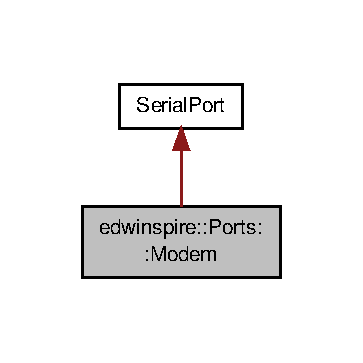
\includegraphics[width=174pt]{classedwinspire_1_1_ports_1_1_modem__inherit__graph}
\end{center}
\end{figure}


Collaboration diagram for edwinspire\-:\-:Ports\-:\-:Modem\-:\nopagebreak
\begin{figure}[H]
\begin{center}
\leavevmode
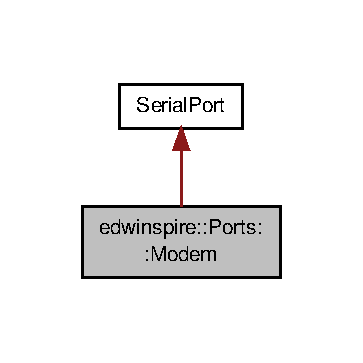
\includegraphics[width=174pt]{classedwinspire_1_1_ports_1_1_modem__coll__graph}
\end{center}
\end{figure}


\subsection{Detailed Description}


Definition at line 94 of file libspire\-\_\-modem\-\_\-new.\-vala.



The documentation for this class was generated from the following file\-:\begin{DoxyCompactItemize}
\item 
libspire\-\_\-modem\-\_\-new.\-vala\end{DoxyCompactItemize}

\hypertarget{classedwinspire_1_1_ports_1_1_response}{\section{edwinspire\-:\-:Ports\-:\-:Response Class Reference}
\label{classedwinspire_1_1_ports_1_1_response}\index{edwinspire\-::\-Ports\-::\-Response@{edwinspire\-::\-Ports\-::\-Response}}
}


Dummy class used for illustration purposes. Doing something with it.  




\subsection{Detailed Description}
Dummy class used for illustration purposes. Doing something with it. 

Detailed description follows here. \begin{DoxyAuthor}{Author}
X. X\-Y\-Z, D\-E\-S\-Y 
\end{DoxyAuthor}
\begin{DoxyDate}{Date}
March 2008 
\end{DoxyDate}


Definition at line 35 of file libspire\-\_\-modem\-\_\-new.\-vala.



The documentation for this class was generated from the following file\-:\begin{DoxyCompactItemize}
\item 
libspire\-\_\-modem\-\_\-new.\-vala\end{DoxyCompactItemize}

\hypertarget{class_serial_port}{\section{Serial\-Port Class Reference}
\label{class_serial_port}\index{Serial\-Port@{Serial\-Port}}
}


Inheritance diagram for Serial\-Port\-:\nopagebreak
\begin{figure}[H]
\begin{center}
\leavevmode
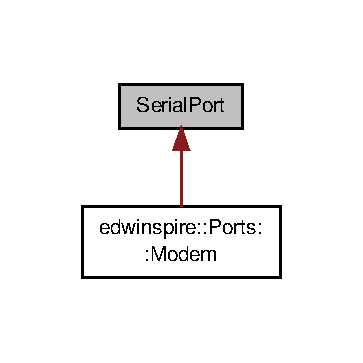
\includegraphics[width=174pt]{class_serial_port__inherit__graph}
\end{center}
\end{figure}


\subsection{Detailed Description}
The \hyperlink{class_serial_port}{Serial\-Port} class contains methods for communications with devices via serial port. 

Definition at line 53 of file libspire\-\_\-serial.\-vala.



The documentation for this class was generated from the following file\-:\begin{DoxyCompactItemize}
\item 
libspire\-\_\-serial.\-vala\end{DoxyCompactItemize}

\printindex
\end{document}
